\section{Energy Models} 

  Now this is the first time we talk about unsupervised learning. Note from our machine learning notes \href{paper.pdf#sec:graphical_models}{here} that for unsupervised tasks, we have estimated the density of complex distributions by factoring them in \textit{graphical models}, e.g. Bayesian networks or Markov random fields. 
  We will extend this into deep learning architectures.\footnote{This is \textit{not} to be confused with graph neural networks (GNNs), which are designed for tasks whose inputs are graphs.} If you are not familiar, you should probably go over graphical models in my ML notes before reading further. 

  Note that many of the theories behind energy models are very old (from the 1980s) and established, especially in the prevalence of the \textit{Boltzmann distribution} in statistical mechanics. All of them essentially rely on the fact that we can model a probability density as 
  \begin{equation}
    p(x) = \frac{e^{-E(x)}}{Z}
  \end{equation}
  for some function $E: \mathbb{R}^n \rightarrow \mathbb{R}$, which we call the \textit{negative energy}, and $Z$ is what we call the \textbf{partition function}. We have seen from the Hammersley-Clifford theorem in my machine learning notes that we can model a joint probability distribution on an undirected graph with the product of potential functions on the max cliques.\footnote{But finding max cliques is NP-hard?} Therefore, we will take advantage of this in the specific instance of MRFs that are \textit{bipartite graphs}, i.e. a non-feedforward (since its cyclic) 2-layer neural network. We will talk about RBMs, deep belief networks, and hopfield networks. Diffusion models, which can also be considered an energy model, will be talked separately. 

  The most straightforward application is that we can just have a neural network approximate this function $E_\theta$, which gives us a parameterized family of distributions $p_\theta (x) = \frac{1}{Z} e^{-E_\theta (x)}$ that would hopefully approximate the true distribution $p^\ast (x)$. This is called an \textbf{energy based model (EBM)}. 

\subsection{Training with MCMC}

  Therefore, we could like to maximize the log-likelihood (which gets rid of the partition function term), giving us 
  \begin{align}
    \argmax_\theta \mathbb{E}_{x \sim p^\ast} \big[ \log p_\theta (x) \big] & = \argmax_\theta \mathbb{E}_{x \sim p^\ast}\big[ -E_\theta (x) \big] - \mathbb{E}_{x \sim p^\ast} \big[ \log{Z_\theta} \big] \\
                                                                            & \approx \argmin_\theta \sum_{i=1}^N E_\theta (x^{(i)}) + \sum_{i=1}^N \log Z_\theta
  \end{align} 
  Note that even though $Z_\theta$ is constantly $1$ with respect to $x$, the actual value of the integral will change with respect to $\theta$. Therefore this term also contributes to the argmax. Focusing on a single sample, we attempt to compute the gradient of this. The first gradient $\nabla_\theta E_\theta (x)$ is easy by automatic differentiation since $E$ is a neural net. However, the second term is quite tricky. But using some mathematical identities mentioned in \cite{ebm_train}, we have 

  \begin{align}
    \nabla_\theta \log Z_\theta & = \nabla_\theta \log \int \exp(-E_\theta(x))dx \\
                                & = \left(\int \exp(-E_\theta(x))dx\right)^{-1} \nabla_\theta \int \exp(-E_\theta(x))dx \\
                                & = \left(\int \exp(-E_\theta(x))dx\right)^{-1} \int \nabla_\theta \exp(-E_\theta(x))dx \\
                                & = \left(\int \exp(-E_\theta(x))dx\right)^{-1} \int \exp(-E_\theta(x))(-\nabla_\theta E_\theta(x))dx \\
                                & = \int \left(\int \exp(-E_\theta(x))dx\right)^{-1} \exp(-E_\theta(x))(-\nabla_\theta E_\theta(x))dx \\
                                & = \int \frac{\exp(-E_\theta(x))}{Z_\theta}(-\nabla_\theta E_\theta(x))dx \\
                                & = \int p_\theta(x)(-\nabla_\theta E_\theta(x))dx \\
                                & = \mathbb{E}_{x\sim p_\theta(x)}[-\nabla_\theta E_\theta(x)]
  \end{align}
  This gives us hope. Therefore, we can estimate the intractable gradient as an expectation of the gradient of the neural network with respect to the current estimate $p_\theta (x)$ (not the true $p^\ast$!). 
  \begin{align}
    \nabla_\theta \mathbb{E}_{x \sim p^\ast} [ \log p_\theta (x)] & = \mathbb{E}_{x \sim p^\ast} [ \nabla_\theta \log p_\theta (x) ] \\
                                                                  & \approx \sum_{i=1}^N - \nabla_\theta E_\theta (x) - \nabla_\theta \log Z_\theta \\
                                                                  & = \sum_{i=1}^N \Big\{ -\nabla_\theta E_\theta (x) + \mathbb{E}_{x \sim p_\theta (x)} [ \nabla_\theta E_\theta (x)] \Big\} \\
                                                                  & \approx \sum_{i=1}^N \bigg\{ -\nabla_\theta E_\theta (x) +  \sum_{j=1}^M \nabla_\theta E_\theta (\Tilde{x}) \bigg\}
  \end{align}
  where the final step is from using a Monte Carlo sample with a size $M$ batch of $\Tilde{x}$ from $p_\theta (x)$. We can draw samples using MCMC, with Langevin dynamics MCMC being the most popular. 

\subsection{Score Matching}

  We have built several types of generative models so far that estimated densities. While calculating PDFs is called \textit{density estimation}, we can indirectly estimate it by calculating the gradient of the PDF (with respect to the sample), which is known as \textbf{score matching}. 

  \begin{definition}[Score]
    Let $X$ be a continuous random variable defined on $\mathbb{R}^n$, and let $p$ be its pdf, parameterized by $\theta$. The score function of $p$ is the gradient of the log-pdf with respect to the sample.\footnote{Note that this is w.r.t. the sample, not the parameter, unlike what we do usually in machine learning.}
    \begin{equation}
      \psi (x; \theta) = \begin{bmatrix} \frac{\partial \log{p(x;\theta)}}{\partial x_1} \\ \vdots \\ \frac{\partial \log{p(x;\theta)}}{\partial x_n} \end{bmatrix} =  
      \begin{bmatrix}
        \psi_1 (x;\theta) \\ \vdots \\ \psi_n (x;\theta)
      \end{bmatrix} = 
      \nabla_x \log{p (x; \theta)}
    \end{equation}
    Note that the score is a function $\psi: \mathbb{R}^n \rightarrow \mathbb{R}^n$. 
  \end{definition} 

  The reason Hyvarinen introduced this score function in 2005 is because we want to have such a score is that it does not depend on the normalizing constant $Z$ (since the log derivative gets rid of it). \cite{orig_score} Therefore, rather than maximizing the likelihood, we want to minimize the L2 distance between the score functions. 

  \begin{equation}
    R(\theta) = \mathbb{E}_{X} \big[ || \psi(x\;\theta) - \psi_{\mathcal{D}} (x) ||^2 \big]
  \end{equation}

  \cite{score}. 

  Note that Fisher score is a number. They use the same notation $s$ to denote gradient of log of the distribution, which is confusing. 

  The relationship is the dual prime inequality, aka 2nd law of thermodynamics. 
  \begin{equation}
    \lim_{t \rightarrow 0} \frac{D_{KL}(p_t || q_t) - D_{KL}(p||q)}{t}
  \end{equation}
  
\subsection{Boltzmann Machines}  

  Okay, so we've learned to model an arbitrary distribution by approximating it with an energy model. While they are not explicitly build into energy models, it is possible to include them. One such method is through \textit{Boltzmann machines}. Consider the graph $x_1, \ldots, x_D$ which represents a random vector $x$ for which we would like to model the probability distribution of. 
  \begin{center}
    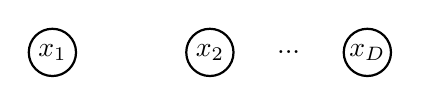
\begin{tikzpicture}
      \node (x1) at (0,0) {$x_1$};
      \node (x2) at (2,0) {$x_2$};
      \node (xD) at (4,0) {$x_D$};

      \node at (3,0) {...};
      \draw[thick] (x1) circle (0.3);
      \draw[thick] (x2) circle (0.3);
      \draw[thick] (xD) circle (0.3);
    \end{tikzpicture}
  \end{center}
  What we can do is model the dependencies between these random elements with linear parameters $W$ and $b$, which essentially gives us a Markov Random Field. Let's consider when $x_i$'s are all Bernoulli, so $x \in \{0, 1\}^D$, which are known as \textit{Ising models} in statistical mechanics. By Hammersley-Clifford, we don't even need to specify the individual functions over the maximal cliques, and rather we can just specify the energy function $E(x)$ of the Boltzmann distribution that the MRF encodes. We parameterize $\theta = \{W, b\}$. 

  \begin{example}[Bernoulli Pairwise Markov Random Fields]
    We define it to capture the interactions between Bernoulli random variables $x_i$ up to order $2$. 
    \begin{equation}
      p_{\theta} (x) = \frac{1}{Z} \exp( E(x)) = \frac{1}{Z} \exp \bigg( \sum_{i j \in E} x_i x_j W_{ij} + \sum_{i \in V} x_i b_i \bigg) = \frac{1}{Z} \exp \big( x^T W x + b^T x \big)
    \end{equation}
    Now let's check its conditional distribution. Let $x_{-k}$ denote the joint distribution of all random variables minus $x_k$.  
    \begin{align}
      p(x_k = 1 \mid x_{-k}) & = \frac{p(x_k = 1, x_{-k})}{p(x_{-k})} \\
                             & = \frac{p(x_k = 1, x_{-k})}{p(x_k = 0, x_{-k}) + p(x_k = 1, x_{-k})} \\
                             & = \frac{\exp \Big( \sum_{k j \in E} x_j W_{kj} + x_k b_k \Big)}{\exp(0) + \exp \Big(\sum_{k j \in E} x_j W_{kj} + x_k b_k \Big)} \\
                             & = \sigma \bigg\{ - b_k x_k - \sum_{k j \in E} x_j W_{k j} \bigg\} 
    \end{align}
    where the penultimate step comes from evaluating 
    \begin{align} 
      p(x_k = 1, x_{-k}) & = \frac{1}{Z(\theta)} \exp \bigg( \sum_{ij \in E, k \neq i, j} x_i x_j W_{ij} + \sum_{i j \in E, k = i, j} x_i x_j W_{ij} + \sum_{i \in V, i \neq k} x_i b_i + x_k b_k \bigg) \\
                         & =\frac{1}{Z(\theta)} \exp \bigg( \sum_{ij \in E, k \neq i, j} x_i x_j W_{ij} + \sum_{k j \in E} x_j W_{kj} + \sum_{i \in V, i \neq k} x_i b_i + b_k \bigg)  \\ 
      p(x_k = 0, x_{-k}) & = \frac{1}{Z(\theta)} \exp \bigg( \sum_{ij \in E, k \neq i, j} x_i x_j W_{ij} + \sum_{i \in V, i \neq k} x_i b_i\bigg)  
    \end{align}
    and canceling out like terms in the numerator and denominator. This tells us that MRFs are related to logistic function.  
  \end{example}

  \begin{example}[Gaussian Markov Random Fields] 
    If we assume that $p_{\theta} (x)$ follows a multivariate Gaussian distribution, we have 
    \begin{equation}
      p(x \mid \mu, \Sigma) = \frac{1}{Z} \exp \bigg( -\frac{1}{2} (x - \mu)^T \Sigma^{-1} (x - \mu) \bigg)
    \end{equation}
    Since the Gaussian distribution represents at most second-order relationships, it automatically encodes a pairwise MRF. Therefore, we can rewrite 
    \begin{equation}
      p(x) = \frac{1}{Z} \exp \bigg( -\frac{1}{2} x^T Jx + g^T x \bigg)
    \end{equation}
    where $J = \Sigma^{-1}$ and $\mu = J^{-1} g$. 
  \end{example}

  However, this is still quite a limited model. For one, due to the linearity of the weight matrix, it always turns out that the probability of $x_k = 1$ is always given by a linear model (logistic regression) from the values of the other units. This family of distributions parameterized by $\theta = \{W, b\}$ may not be broad enough to capture the true $p(x)$. Therefore, we can add latent variables that can act similarly to hidden units in a MLP and model higher-order interactions among the visible units. Just as the addition of hidden units to convert logistic regression into MLP results in the MLP being a universal approximator of functions, a Boltzmann machine with hidden units is not longer limited to modeling linear relationships between variables. Instead, the Boltzmann machine becomes a universal approximator of probability mass functions over discrete random variables. 

  \begin{definition}[Boltzmann Machine]
    The original \textbf{Boltzmann machine} has the energy function 
    \begin{equation}
      E(v, h) = - v^T R v - v^T W h - h^T S h - b^T v - c^T h
    \end{equation}
    It can represent the undirected graph that has connections within the $x$, within the $h$, and between the $x$ and $h$.

    \begin{figure}[H]
      \centering 
      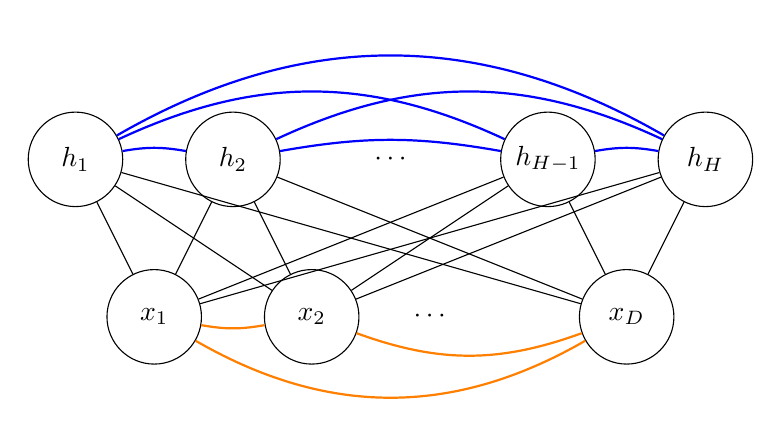
\begin{tikzpicture}[
        node/.style={circle, draw, minimum size=1.2cm},
        every edge/.style={draw, -}
      ]
        % Create h nodes (top layer)
        \node[node] (h1) at (0,2) {$h_1$};
        \node[node] (h2) at (2,2) {$h_2$};
        \node at (4,2) {$\cdots$};
        \node[node] (hm1) at (6,2) {$h_{H-1}$};
        \node[node] (hH) at (8,2) {$h_H$};

        % Create x nodes (bottom layer)
        \node[node] (x1) at (1,0) {$x_1$};
        \node[node] (x2) at (3,0) {$x_2$};
        \node at (4.5,0) {$\cdots$};
        \node[node] (xD) at (7,0) {$x_D$};

        % Draw connections between layers
        \foreach \i in {1,2,m1,H} {
            \foreach \j in {1,2,D} {
              \draw (h\i) -- (x\j);
            }
        }

        % Draw the blue arc on top
        \draw[blue, thick] (h1) to[bend left=30] node[above] {} (hH);
        \draw[blue, thick] (h1) to[bend left=10] node[above] {} (h2);
        \draw[blue, thick] (h1) to[bend left=25] node[above] {} (hm1);
        \draw[blue, thick] (hm1) to[bend left=10] node[above] {} (hH);
        \draw[blue, thick] (h2) to[bend left=10] node[above] {} (hm1);
        \draw[blue, thick] (h2) to[bend left=25] node[above] {} (hH);

        % Draw the orange arc on bottom
        \draw[orange, thick] (x1) to[bend right=30] node[below] {} (xD);
        \draw[orange, thick] (x1) to[bend right=10] node[below] {} (x2);
        \draw[orange, thick] (x2) to[bend right=20] node[below] {} (xD);
      \end{tikzpicture}
      \caption{2-layer undirected graph representing a Boltzmann machine. } 
      \label{fig:boltzmann}
    \end{figure}
  \end{definition} 

  Therefore, by adding latent variables and connecting everything together, this gives us a very flexible model that can capture a lot of distributions.  

\subsection{Restricted Boltzmann Machines} 

  Unfortunately, there are problems with training this, and so the restricted Boltzmann machine allowed for efficient training. Therefore, we will limit ourselves to \textbf{pairwise MRFs}, which only capture dependencies between cliques of maximum size $2$. We usually write $x$ as the observed and $z$ as the latent, but in the literature $v$ and $h$ are used, respectively. Now, if we put a restriction saying that there cannot be any intra-connections in the $x$ and $h$, then we get the \textit{restricted Boltzmann machine}, which has a slightly more resticted form of the energy function than the general BM. 

  \begin{definition}[Restricted Boltzmann Machine] 
    The \textbf{restricted Boltzmann machine} has the energy function 
    \begin{equation}
      E(v, h) = - v^T W h - b^T v - c^T h
    \end{equation}
    with connections only allowed between $x_i$'s and $h_j$'s, known as a \textbf{bipartite graph}, implying that the maximum clique length is $2$. This model allows the elements of $x$ to be dependent, but this architecture allows for \textit{conditional independence}, and not just for $x$ given $h$, but also $h$ given $x$. Therefore, we already have the extremely nice property that 
    \begin{align} 
      p(x \mid h) & = \prod_{k=1}^{D} p(x_k \mid h) \\
      p(h \mid x) & = \prod_{j=1}^F p(h_j \mid x) 
    \end{align}

    \begin{figure}[H]
      \centering 
      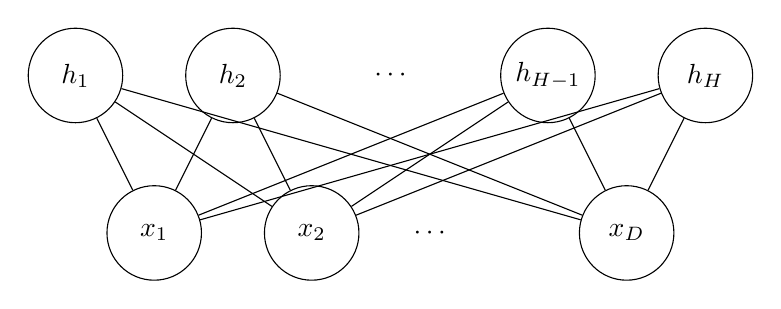
\begin{tikzpicture}[
        node/.style={circle, draw, minimum size=1.2cm},
        every edge/.style={draw, -}
      ]
        % Create h nodes (top layer)
        \node[node] (h1) at (0,2) {$h_1$};
        \node[node] (h2) at (2,2) {$h_2$};
        \node at (4,2) {$\cdots$};
        \node[node] (hm1) at (6,2) {$h_{H-1}$};
        \node[node] (hH) at (8,2) {$h_H$};

        % Create x nodes (bottom layer)
        \node[node] (x1) at (1,0) {$x_1$};
        \node[node] (x2) at (3,0) {$x_2$};
        \node at (4.5,0) {$\cdots$};
        \node[node] (xD) at (7,0) {$x_D$};

        % Draw connections between layers
        \foreach \i in {1,2,m1,H} {
            \foreach \j in {1,2,D} {
              \draw (h\i) -- (x\j);
            }
        }
      \end{tikzpicture}
      \caption{2-layer undirected graph representing a restricted Boltzmann machine. Note that the intra-connections (blue and orange) are gone. } 
      \label{fig:rbm}
    \end{figure}
  \end{definition}

  Note that this form of the probability $E(x)$ is equivalent to the product of max-cliques, which are of size 2 in this case. 
  \begin{align}
    p(v, h) & = \exp(-E(v, h)) / Z \\ 
            & = \exp(v^T W h + b^T v + c^T h) / Z \\
            & = \exp(v^T W h) \exp(b^T v) \exp (c^T h) / Z  \\
            & = \frac{1}{Z} \prod_j \prod_k \exp(W_{jk} h_j v_k) \, \prod_k \exp(c_k v_k) \, \prod_j \exp(b_j h_j)
  \end{align}
  Therefore, we can think of the $\exp(h^T W x)$ as encoding the cliques of length $2$ and the others as cliques of length $1$. The fact that we can calculate $p(h \mid x)$ means that inferring the distribution over the hidden variables is easy. 

  \subsubsection{Contrastive Divergence}

    Now that we've done this, we can finally get to training the model. Now, essentially this is density estimation problem given dataset $\mathcal{D} = \{x^{(t)}\}$ of iid random variables, we want to maximize the likelihood of $p_{\theta}$, which is really just equivalent to optimizing $E_{\theta}$. So, let's take the average negative log-likelihood and take the derivative of it
    \begin{equation}
      \frac{\partial}{\partial \theta} \frac{1}{T} \sum_t - \log p_{\theta} (x^{(t)})
    \end{equation}
    There's a lot of computation to do here, so let's focus on one sample $x^{(t)}$ and claim that the gradient ultimately ends up as the following. 

    \begin{theorem}[Decomposition of Derivative]
      The derivative of the log-likelihood decomposes into the following terms. 
      \begin{align} 
        \frac{\partial}{\partial \theta} - \log p(x^{(t)}) & = \sum_{h}  p(h \mid x^{(t)}) \, \frac{ \partial E(x^{(t)}, h)}{\partial \theta} - \sum_{x, h} p(x, h) \, \frac{\partial E(x, h)}{\partial \theta} \\
                                                           & = \underbrace{\mathbb{E}_{h} \bigg[ \frac{\partial E( x^{(t)}, h)}{\partial \theta} \; \bigg| \; x^{(t)} \bigg]}_{\text{positive phase}} - \underbrace{\mathbb{E}_{x, h} \bigg[ \frac{\partial E(x, h)}{\partial \theta} \bigg]}_{\text{negative phase}}
      \end{align}
      which reduces to 
      \begin{equation}
        -\nabla_\theta \ln{p(x)} = \begin{cases}
          - \nabla_W \ln{p(x)} & = \sum_h p(h \mid x) h x^T - \sum_{x, h} p(x, h) h x^T \\
          - \nabla_b \ln{p(x)} & =  \sum_h p(h \mid x) h - \sum_{x, h} p(x, h) h \\
          - \nabla_c \ln{p(x)} & =  \sum_h p(h \mid x) x - \sum_{x, h} p(x, h) x
        \end{cases}
      \end{equation}
    \end{theorem}
    \begin{proof}
      From the energy model form, we can see that $Z = \sum_{x, h} \exp(-E(x, h))$. Therefore, 
      \begin{align}
        \ln(Z) & = \ln \bigg( \sum_{x, h} \exp(-E(x, h)) \bigg) \\ 
        \frac{\partial}{\partial \theta} \ln(Z) & = \frac{1}{Z} \sum_{x, h} \exp(-E(x, h)) \cdot -1 \cdot \frac{\partial}{\partial \theta} E(x, h) \\
               & = -\frac{1}{Z} \sum_{x, h} \exp(-E(x, h)) \cdot \frac{\partial}{\partial \theta} E(x, h) \\
               & = -\frac{1}{Z} \sum_{x, h} Z \cdot p(x, h) \cdot \frac{\partial}{\partial \theta} E(x, h) \\
               & = - \sum_{x, h} p(x, h) \frac{\partial E(x, h)}{\partial \theta}
      \end{align}
      We have by definition 
      \begin{equation} 
        -\ln p(x) = - \ln \bigg\{ \sum_{h} \exp \big( -E(x, h) \big) \bigg\} + \ln(Z)
      \end{equation}
      and so when taking the derivative, the second term is solved from above and the first term, we apply the chain rule to get 
      \begin{align} 
        -\frac{\partial}{\partial \theta} \ln p(x) & = \frac{\sum_{h} \exp \big( -E(x, h) \big) \, \frac{\partial E(x, h)}{\partial \theta} / Z}{\sum_{h} \exp \big( -E (x, h) \big) / Z} + \frac{\partial \ln(Z)}{\partial \theta} \\
                                                                         & = \frac{\sum_{h} p(x, h) \, \frac{\partial E(x, h)}{\partial \theta}}{p(x)} + \frac{\partial \ln(Z)}{\partial \theta} \\
                                                                         & = \sum_{h} p(h \mid x) \, \frac{\partial E(x, h)}{\partial \theta} - \sum_{x, h} p(x, h) \, \frac{\partial E(x, h)}{\partial \theta} 
      \end{align} 
      We can use the closed form of $E$ to then compute its partials. 
      \begin{align}
        \bigg( \frac{\partial E(x, h)}{\partial W} \bigg)_{ij} & = \frac{\partial E(x, h)}{\partial W_{ij}} = \frac{\partial}{\partial W_{ij}} \bigg\{ - \sum_{i,j} W_{ij} h_i x_j - \sum_j c_j x_j - \sum_i b_i h_i \bigg\} = h_i x_j \\
        \bigg( \frac{\partial E(x, h)}{\partial b} \bigg)_i & = \frac{\partial E(x, h)}{\partial b_i} = h_i  \\
        \bigg( \frac{\partial E(x, h)}{\partial c} \bigg)_j & = \frac{\partial E(x, h)}{\partial c_j} = x_j 
      \end{align}  
      which in matrix form is 
      \begin{align}
        \nabla_{\theta} E(x, h) = \{ \nabla_W E(x, h), \nabla_b E(x, h), \nabla_c E(x, h) \} = \{ h x^T, h, x \}
      \end{align}
      The conditional probability can be factorized out given $x$ and computed easily by conditional independence. 
      \begin{equation}
        p(h \mid x) = \prod_j p(h_j \mid x)
      \end{equation}
      and so given that we have computed this for all $h$, we can write our gradient as 
      \begin{equation}
        -\nabla_\theta \ln{p(x)} = \begin{cases}
          - \nabla_W \ln{p(x)} & = \sum_h p(h \mid x) h x^T - \sum_{x, h} p(x, h) h x^T \\
          - \nabla_b \ln{p(x)} & =  \sum_h p(h \mid x) h - \sum_{x, h} p(x, h) h \\
          - \nabla_c \ln{p(x)} & =  \sum_h p(h \mid x) x - \sum_{x, h} p(x, h) x
        \end{cases}
      \end{equation}
    \end{proof} 

    Therefore, we can easily compute the left summation in the gradient form, but the right summation requires us to compute $p(x, h)$ as a general joint distribution, which is intractable. So we just approximate this with a Monte Carlo estimator, specifically Gibbs sampling. This method is known as \textit{contrastive divergence} which was introduced in 2002 by Geoffrey Hinton in \cite{cd}. 

    \begin{algo}[Contrastive Divergence] 
      The general idea is to replace by the expectation by a point estimate at $\Tilde{x}$, which we can obtain by sampling the conditions over and over through Gibbs. Since we know $p(x\mid h)$ and $p(h \mid x)$ easily, we can start sampling the chain for some predetermined $K$ steps (actually $2K$ since we are sampling the $x$ and $h$ back and forth), and whatever $\Tilde{x}, \Tilde{h}$ you sample at the end is your estimate. You then use this to approximate the negative phase 
      \begin{equation}
        \mathbb{E}_{x, h} \bigg[ \frac{\partial E(x, h)}{\partial \theta} \bigg] \approx \frac{\partial}{\partial \theta} E(\Tilde{x}, \Tilde{h})
      \end{equation}
      Here are the steps. 
      \begin{enumerate}
        \item Initialize $x^0 = x$ and sample $h^0$ from $p(h \mid x^0)$. 
        \item For $k = 1, \ldots, K$, 
        \begin{enumerate}
          \item Sample $x^k$ from $p(x \mid h^{k-1})$. 
          \item Sample $h^k$ from $p(h \mid x^k)$. 
        \end{enumerate}
        \item Once you get $\Tilde{x} = x^K$,\footnote{Note that we do not use $\Tilde{h} = h^K$.} use this to approximate 
        \begin{align}
          - \nabla_W \ln{p(x)} & = \sum_h p(h \mid x) h x^T - \sum_{x, h} p(x, h) h x^T && \approx \sum_h p(h \mid x) h x^T - \sum_h p(h \mid \Tilde{x}) h \Tilde{x}^T \\
          - \nabla_b \ln{p(x)} & =  \sum_h p(h \mid x) h - \sum_{x, h} p(x, h) h && \approx \sum_h p(h \mid x) h - \sum_h p(h \mid \Tilde{x}) h \\
          - \nabla_c \ln{p(x)} & =  \sum_h p(h \mid x) x - \sum_{x, h} p(x, h) x && \approx \sum_h p(h \mid x) x - \sum_h p(h \mid \Tilde{x}) \Tilde{x}
        \end{align}
      \end{enumerate}

      We can tweak this procedure, such as \textbf{persistent CD}, where instead of initializing the chain to $x^{(t)}$, we can initialize the chain to the negative sample of the last iteration. 

      \begin{figure}[H]
        \centering 
        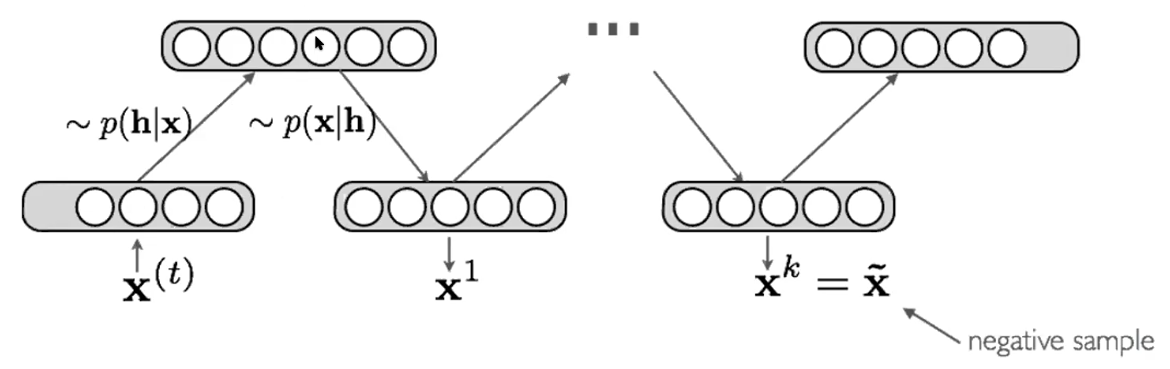
\includegraphics[scale=0.4]{img/contrastive_divergence.png}
        \caption{In general, the bigger $k$ is, the less biased the estimate of the gradient will be, and in practice $k=1$ works well for learning good features. The reason this is called contrastive divergence is that in the gradient update step, we have a positive sample and a negative sample that both approximates the expected gradient, which contrasts to each other. }
        \label{fig:contrastive_divergence}
      \end{figure}
      Therefore, contrastive divergence with $k$ iterations gives us the \textbf{CD-k algorithm}. 
    \end{algo}

    \begin{algo}[Fitting]
      Therefore, for updating $\theta$, we get the following 
      \begin{align} 
        W & = W - \alpha \big( \nabla_{W}(- \log p(x^{(t)})) \big) \\
                   & = W - \alpha \big( \mathbb{E}_{h} [ \nabla_{W} E(x^{(t)}, h) \mid x^{(t)} ] - \mathbb{E}_{x, h} [\nabla_{W} E(x, h) ]\big) \\
                   & = W - \alpha \big( \mathbb{E}_{h} [ \nabla_{W} E(x^{(t)}, h) \mid x^{(t)} ] - \mathbb{E}_{h} [\nabla_{W} E(\bar{x}, h) \mid \bar{x} ]\big) \\
                   & = W + \alpha \big( h(x^{(t)}) (x^{(t)})^T               - h(\bar{x}) \bar{x}^T \big)
      \end{align}
      and doing this over all three parameters leads to 
      \begin{align} 
        W & \leftarrow W + \alpha \big( h (x^{(t)}) (x^{(t)})^T - h(\bar{x}) \bar{x}^T \big) \\
        b & \leftarrow b + \alpha \big( h(x^{(t)}) - h(\bar{x}) \big) \\
        c & = \leftarrow c + \alpha \big( x^{(t)} - \hat{x} \big) 
      \end{align}
    \end{algo} 

    \begin{example}[Collaborative Filtering]
      Netflix dataset. 
    \end{example}

  \subsubsection{Inference with Bernoulli-Bernoulli RBMs}

    We have talked about RBMs of a general form, but the standard is that the hidden units are almost always Bernoulli, while the visible ones are either Bernoulli or Gaussian. Let's talk about when $x, h$ are both Bernoulli, which allows us to simplify the general form of training. 

    \begin{definition}[Bernoulli-Bernoulli RBM]
      For now, let us assume that we are trying to estimate the distribution of a Bernoulli random vector $x \in \{0, 1\}^D$ with Bernoulli latent variables $h \in \{0, 1\}^F$. Then, the energy of the joint configuration is  
      \begin{equation}
        E(v, h; \theta) = - \sum_{ij} W_{ij} v_i h_j - \sum_i b_i v_i - \sum_j a_j h_j = - v^T W h - b^T v - a^T h
      \end{equation}
      where $\theta = \{W, a, b\}$ are the model parameters. 
    \end{definition}

    Let's get some calculations out of the way. 

    \begin{lemma}[Conditional Distributions] 
      For the Bernoulli RBM, we have 
      \begin{align} 
        p(h_j = 1 \mid x) & = \sigma ( b_j + W_{j,:} x) \\
        p(x_k = 1 \mid h) & = \sigma ( c_k + h^T W_{:, k})
      \end{align}
    \end{lemma}
    \begin{proof}
      Just use the definition of conditional probability and substitute the result below in the denominator. The terms will cancel out. 
    \end{proof}

    \begin{lemma}[Free Energy] 
      For the Bernoulli RBM, we want to compute the marginal $p(x)$ as
      \begin{align*} 
      p(x) & = \frac{\exp(-F(x))}{Z} \\
                    & = \frac{1}{Z} \exp \bigg( c^T x + \sum_{j=1}^H \log \big( 1 + \exp (b_j + W_{j, :} x) \big) \bigg) \\
                    & = \frac{1}{Z} \exp \bigg( c^T x + \sum_{j=1}^H \mathrm{softplus}(b_j + W_{j, :} x ) \bigg)
      \end{align*}
      where $F$ is called the \textbf{free energy} and the softplus is defined. 
      \begin{equation}
        \text{softplus}(x) = \ln(1 + e^x)
      \end{equation}
      Therefore, $p(x)$ is calculated by taking the product of these terms, which is why it's known as a \textbf{product of experts model}. 

      \begin{figure}[H]
        \centering 
        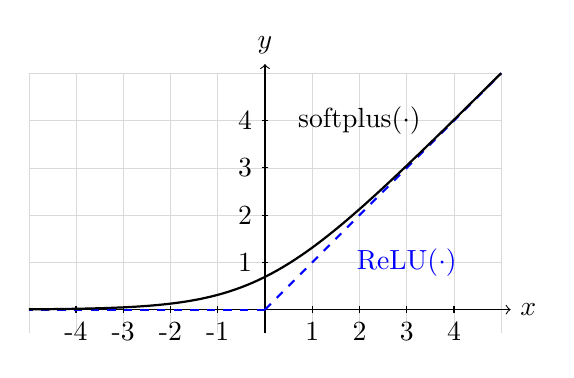
\begin{tikzpicture}[
          scale=0.6,
          declare function={
              softplus(\x) = ln(1 + exp(\x));
          }
        ]
          % Grid and axes
          \draw[very thin,gray!30] (-5,-0.5) grid (5,5);
          \draw[->] (-5,0) -- (5.2,0) node[right] {$x$};
          \draw[->] (0,-0.5) -- (0,5.2) node[above] {$y$};

          % Tick marks
          \foreach \x in {-4,-3,-2,-1,1,2,3,4} {
              \draw (\x,2pt) -- (\x,-2pt) node[below] {\x};
          }
          \foreach \y in {1,2,3,4} {
              \draw (2pt,\y) -- (-2pt,\y) node[left] {\y};
          }

          % Function label
          \node at (2,4) {softplus($\cdot$)};
          \node[blue] at (3,1) {ReLU($\cdot$)};

          % Dashed line (identity function after x>0)
          \draw[thick, blue, dashed] (0,0) -- (5,5);
          \draw[thick, blue, dashed] (0,0) -- (-5,0);

          % Softplus function
          \draw[thick] plot[domain=-5:5, samples=100] (\x,{softplus(\x)});
        \end{tikzpicture}
        \caption{A graph of the softplus activation function, with the dotted ReLU.} 
        \label{fig:softplus}
      \end{figure}
    \end{lemma}
    \begin{proof}
      We have 
      \begin{align} 
        p(x) & = \sum_{h \in \{0, 1\}^H} \exp \big( h W x + c^T x + b^T h\big) /Z \\
                      & = \exp (c^T x) \sum_{h_1 = 0, 1} \ldots \sum_{h_H = 0, 1} \exp \bigg( \sum_j h_j W_{j, :} x + b_j h_j \bigg) / Z \\
                      & = \exp (c^T x) \bigg( \sum_{h_1 = 0, 1} \exp (h_1 W_{1, :} x + b_1 h_1 ) \bigg) \ldots \bigg( \sum_{h_H = 0, 1} \exp (h_H W_{H, :} x + b_H h_H) \bigg) / Z \\
                      & = \exp (c^T x) \big( 1 + \exp (b_1 + W_{1, :} x) \big) \ldots \big( 1 + \exp (b_H + W_{H, :} x)\big) / Z \\
                      & = \exp (c^T x) \exp\big\{ \log \big( 1 + \exp (b_1 + W_{1, :} x) \big) \big\} \ldots \exp \big\{ \log \big( 1 + \exp (b_H + W_{H, :} x) \big) \big\} / Z \\
                      & = \frac{1}{Z} \exp \bigg( c^T x + \sum_{j=1}^H \log \big( 1 + \exp (b_j + W_{j, :} x) \big) \bigg) 
      \end{align} 
    \end{proof}

    When training, we can use the closed form to simplify our calculations. 
    \begin{equation}
      \frac{\partial E(x, h)}{\partial W_{j k}} = \frac{\partial}{\partial W_{j k}} 
    \end{equation}
    and so 
    \begin{equation}
      \mathbb{E}_{h} \bigg[ \frac{\partial E(x, h)}{\partial W_{j k}} \bigg| x \bigg] = \mathbb{E}_{h} [ -h_j x_k \mid x] = \sum_{h_j = 0, 1} - h_j x_k \, p(h_j \mid x) = - x_k p(h_j = 1 \mid x)
    \end{equation}
    where the final term is a sigmoid. Hence, we have 
    \begin{equation}
      \mathbb{E}_{h} [ \nabla_{W} E(w, h) \mid x] = - h(x) x^T, \text{ where } h(x) \coloneqq \begin{pmatrix} p(h_1 = 1 \mid x) \\ \vdots \\ p(h_H = 1 \mid x) \end{pmatrix} = \sigma(b + W x)
    \end{equation}
    Now we can substitute what we solved into the second expectation, but again this is infeasible to calculate 
    \begin{equation}
      \mathbb{E}_{x, h} \bigg[ \frac{\partial E(x, h)}{\partial\theta}\bigg] = \sum_{x, h} h(x) x^T p(x, h)
    \end{equation}


  \subsubsection{Inference with Gaussian-Bernoulli RBMs}

    Now we can talk about Gaussian Bernoulli RBMs. 

    \begin{definition}[Gaussian-Bernoulli RBM] 
      If we assume that $v$ is a real-valued (unbounded) input that follows a Gaussian distribution (with $h$ still Bernoulli), then we can add a quadratic term to the energy function 
      \begin{equation} 
        E(x, h) = - h^T W x - c^T x - b^T h - \frac{1}{2} x^T x
      \end{equation}
      In this case, $p(x \mid h)$ becomes a Gaussian distribution $N(c + W^T h, I)$. The training process is slightly harder for this, so what we usually do is normalize the training set by subtracting the mean off each input and dividing the input by the training set standard deviation to get  
      \begin{equation} 
        E(v, h; \theta) = \sum_i \frac{(v_i - b_i)^2}{2 \sigma_i^2} - \sum_{ij} W_{ij} h_j \frac{v_i}{\sigma_i} - \sum_j a_j h_j
      \end{equation}
      You should also use a smaller learning rate $\alpha$ compared to Bernoulli RBM. 
    \end{definition} 

    \begin{algo}[Implementation]
      For an implementation with PyTorch, see \href{code/rbm.html}{here}. 
    \end{algo}

\subsection{Deep Belief Network} 

  Proposed in 2006

  So far, BMs and RBMs aren't really \textit{deep} since they are shallow 2-layer networks, and I could have placed them in my machine learning notes in graphical models. However, RBMs provided the foundations for deep belief networks, a pivotal moment in deep learning, and thus they are considered part of the deep learning curriculum. 

\subsection{Hopfield Networks}

  They are EBMs and RNNs!

